\section{Realisierung}
Wie bereits in der Systembeschreibung beschrieben, wird der Fahrsimulator in dei Hauptkomponenten unterteilt. Zum Fahrsimulator gehört ein UDP-Listener, ein Szenen-Manager und das Hauptprogramm. Da die Verbindung zwischen dem Cockpit und dem Fahrsimulator mit einer Netzwerkschnittstelle realisiert wird, ist es möglich die Anbindung an das Cockpit und den Fahrsimulator physisch auf zwei Rechnern zu betreiben. Eine Alternative ist die Umsetzung mit dem Ogre Framwork (Siehe Anhang C). Dieses Framework bietet umfassende Lösungen um Steuerradär und Pedalen, wie sie in userem Cockpit vorhanden sind, anzusteuern.\\
Da die 3D-Umgebung mit fortscheitendem Projekt ausgebaut wird, könnte sich die notwendige Rechenleistung erheblich steigern. Folgen ungenügender Leistung sind unregelmässige Bewegungen (Lags) in der virtuellen Umgebung oder sogar bis zum Absturz des gesamten Programms führen. Dieses Problem hat zur Folge, dass der Fahrsimulator einer hohen Portierbarkeitanforderung genügen muss. \\
Aus diesem Grund ist die erste Variante mit der Netzwerkschnittstelle für das Fahrsimulatorprojekt besser geeignet. Die andere Variante wird verworfen.
\subsection{LabView modifizierung}
Eine LabVIEW-Umgebung existiert bereits auf dem Rechner an dem das Cockpit angeschlossen ist. Dazu existierte ein LabVIEW-Programm, dass bereits die Eingaben im Cockpit einliest. Da dieses Programm jedoch nicht genau den Anforderungen entspricht, wird ein neues LabVIEW-Programm realisiert. Dieses Programm wird so erweitert das diese Eingaben in Form von definierten Parameter als UDP-Packet permanent gesendet werden. Zusätzlich wird ein zweiter UDP-Socket eingerichtet um Packete die vom Fahrsimulator gesendet werden zu empfangen. Die Daten der empfangenen Packete werden von LabVIEW in ein Log-File gespeichert. 
% ev Bild
\subsection{UDP-Socket}
Die Paramter werden vom LabVIEW-Programm permanent gelesen und mindestens 50 mal pro Sekunde wird ein UDP-Packet gesendet. Um die Zeit zwischen der Eingabe des Probanden und derReaktion des Fahrzeuges im Simulator möglichst gering zu halten, müssen ankommende Packete sofort gelesen werden. Angesitchts der hohen Anzahl an Datenpacketen pro Zeitraum, ist es vernachlässigbar, wenn einige Packete verloren gehen oder vertauscht werden. Das UDP-Protokoll gewährleistet genau diese Eigenschaften.

\begin{figure}[htbp]
\centering 
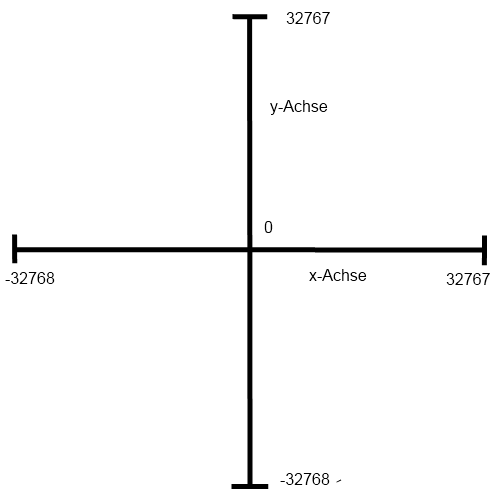
\includegraphics[scale=0.5]{src/koordinatensystem.png}
\caption{Koordinatensystem} % Titel der Grafik
\label{Koordinatensystem} % Labelname
\end{figure}

Die von LabVIEW empfangenen Daten sind in erster Linie Parameter die den Zustand der Pedalen und des Steuerrades representieren. Die beiden Pedalen werden in einem Koordinatensystem wie in Abbildung \ref{Koordinatensystem} auf der y-Achse abgebildet. Die positive y-Richtung quantifiziert das Gas und die negative y-Richtung das Bremspedal. Die Intensität beider Pedalen wird durch 32767 bzw. 32768 ganzzahlige Werte identifiziert. Wenn also keines der beiden Pedalen gedrückt ist, wird dies durch den y-Wert 0 dargestellt. Ein voll gedrücktes Gaspedal entspricht dem y-Wert 32767 und dementsprechend ein voll gedrücktes Bremspedal dem Wert -32768. Der x-Wert im Koordinatensystem quantifiziert den Einschlagswinkel des Steuerrades. Ist das Steuerrad in der neutralen Stellung, entspricht dies dem x-Wert 0. Wenn das Steuerrad vollständig nach rechts eingeschlagen ist, wird dies durch den positiven x-Wert 32767 identifiziert. Umgekehrt wird ein vollständiger Einschlag nach links durch den negativen x-Wert -32768 identifiziert. Es können zusätzlich weitere Parameter wie Tastendrücke am Steuerrad, übermittelt werden, wenn dies erforderlich sein sollte. Zusätzlich zu den Parametern des Cockpits wird von LabVIEW auch noch ein Timestamp gesendet. Der Timestamp wird von UDP-Listener empfangen und nach dem Abspeichern der Parameter wieder zurückgeschickt. Somit kann festgestellt werden, wieviel Verzögerung die Netzwerkschnittstelle verursacht. \\
Da das LabVIEW-Programm und der Simulator nicht synchronisiert sind, wird der DP-Listener zur Überbrückung verwendet. Der UDP-Listener speichert alle Parameter in Variabeln ab. Diese Variabeln werden vom Hauptprogramm ausgelesen und interpretiert. Dieses auslesen der Variabeln erfolgt nun synchron, da das Hauptprogramm nur dann Daten vom UDP-Listener liest, wenn dieses dazu bereit ist.

\subsection{Virtual Reality}
Eine erste Idee um eine virtuelle Realität zu erzeugen, war ein Einsatz von google Street View oder google Maps. Google Maps bietet die möglichkeit, da die Satelitenbilder von der ganzen Erde gemacht wurden, überall auf der Welt zu fahren. Jedoch ist die Auflösung der Bilder nicht immer genug hoch um diese aus der Sicht eines Fahrers anzeigen zu können. Erschwerend kommt hinzu, dass die Aufnahmen nur von oben gemacht wurden und somit keine Seitenansicht einer steilen Felswand oder eines Hauses zur verfügung steht. Auch werden, da die Fotos aus der Vogelperspektive gemacht wurden, verschiedene Elemente die sich über der Strasse befinden wie zum Beispiel Bäume, Brücken oder Autos auf der Strasse flachgedrückt angezeigt.  Dies bedeutet das kein klare Strasse sichtbar ist. Somit wäre der Einsatz von google maps keine zufriedenstellende Lösung. \\
Eine bessere Auflösung und darstellung der Strassen bietet Google Street View. Hierbei wurd mit einem Wagen, der eine 360 Grad Kamera auf dem Dach montiert hatte, den Strassen entlang gefahren und ca. alle 20 Meter ein Foto gemacht. An einem solchen Punkt an dem ein Foto gemacht wurde, kann der Benutzer nun in alle Richtungen Blicken. Es werden sogar grosse Gegenstände wie Wände oder Hausmauern erkannt und beim drehen der Ansicht interpoliert. Diese interpolierung ist jedoch nicht immer korrekt und führt teilweise zu merkwürdigen Anzeigen. Zudem gibt es zwischen zwei Bildern einen zu grossen Unterschied um eine fliesende Bewegung zu Simulieren. Dies könnte durch eine Interpolation der zwei Bilder gelöst werden was viel Rechenleistung kostet und denoch ein unbefriedigendes Resultat liefert. Denn durch die Interpolation wird die Lücke zwischen den beiden Bildern zwar aufgefüllt, jedoch ist der Übergang derart verschwommen das keine Objekte erkannt werden können. 
%ev. Screenshot
Zudem wurden meist nur auf einer Spur Fotos gemacht. Eine Ausnahme bilden die Autobahnen. Auf allen übrigen Strassen hat man sich darauf beschränkt Fotos nur in eine Richtung zu machen. Wenn man nun in die andere Richtung fahren möchte, sieht es so aus als würde man auf der falschen Seite fahren. Somit kommen einem die anderen Verkehrsteilnehmer, die sich ebenfalls auf den Fotos befinden, entgegen. Auch dieser Lösungsansatz muss deshalb Verworfen werden. Eine weiter möglichkeit besteht darin, dass eine eingene Umgebung entworfen wird.\\
Für den Fahrsimulator wird also eine virtuelle dreidimensionale Umgebung benötigt, in der man sich bewegen kann. Diese Umgebung, auch Szene genannt, setzt sich aus verschiedenen Objekten zusammen. Die Struktur eines solchen Objektes wird duch ein Mesh-File beschrieben. In einer Szene kann das gleiche Objekt mehrmals an verschiedenen Positionen vorkommen. Das Objekt kann durch eine skalierung auch einmal gross und einmal klein erscheinen. Oder man kann sie durch eine Rotation unterschiedlich machen. Zusätzlich wird mindestens ein Material-File benötigt in dem sämtliche Texturen und Materialien, die von Objekten der Szene verwendet werden, definiert sind.
Ein Beispiel von einem Matrial wie es ein einem material-File definiert ist wird im Listing \ref{example_materialfile_material} illustriert.
\begin{lstlisting}[caption={Beispiel aus dem material-File für ein Material},label={example_materialfile_material}]
material city_ground
{
	technique
	{
		pass
		{
			diffuse 0.0 0.0 0.0 1.00
			ambient 0.75 0.75 0.75 1.00	
		}
	}
}
\end{lstlisting}
Nach dem Keyword \textit{material} wird der Name des Materials angegeben. Als \textit{technique}-Block wird hier einer angegeben. Es können mehrere Blöcke angegeben. Diese Blöcke können optional auch Namen gegeben werden um zu identifizieren wofür die einzelnen Blöcke sind. Ausgeführt wird jedoch immer nur einer der Blöcke wobei der erste Block der bevorzugteste ist und der unterste Block die letzte Fallbacklösung wäre. Im \textit{pass}-Block werden die Reflektionswerte und die Farbe angegeben. Es können mehrer \textit{pass}-Blöcke angegeben werden die jeweils hintereinander ausgeführt werden und sich überlagern. Das \textit{ambiant} als ambientes Licht bestimmt grundsätzlich die Farbe des Matierials. Die Zahlen repräsentieren die RGB-Werte und können zwischen 0 und 1 liegen. Die Farbe des Materials in diesem Beispiel ist ein helles Grau. Die vierte Zahl representiert den Alphawert der Farbe. Der Alphawert quantifiziert die Sichtbarkeit des Materials wobei 1.0 voll sichtbar und 0.0 unsichtbar ist. \\

Weiter zeigt das Listing \ref{example_materialfile_texture} die definition einer Textur in einem material-File.
\begin{lstlisting}[caption={Beispiel aus dem material-File für eine Textur},label={example_materialfile_texture}]
material city_street_h
{
	technique
	{
		pass
		{
			diffuse 0.80 0.80 0.80 1.00

			texture_unit
			{
				texture street_h.png 2d 4
				filtering anisotropic
			}
		}
	}
}
\end{lstlisting}
Für die Textur wird in diesem Beispiel kein Ambientes Licht definiert und es wird der Standartwert 0 genommen. Der diffuse Anteil bestimmt wie stark das Material das Licht reflektiert. Da die Textur des Materials gut sichtbar sein soll, fällt dieser Wert relativ hoch aus. Im Block \textit{texture\_unit} wird die Textur angegeben und konfiguriert. Die Graphik die als Textur verwendet wird, wird nach dem Keyword \textit{texture} angegeben. Das erster Argument nach der Graphikdatei, das \textit{2d} konfiguriert die zweidimensionale Graphik als normale zweidimensionale Textur. Die vier als drittes Argument gibt die Anzahl zu generierenden Mipmaps an. Zusätzlich kann ein Filter für die Textur mit dem Keyword \textit{filtering} angegeben werden. Der anisotropische Filter wertet die Qualität der Textur in der Distanz auf. Hierbei wird die Richtung, der die Textur betrachtet wird, berücksichtigt.\\
Es werden zwei unterschiedliche Szenen für den Fahrsimulator erstellt. Die eine Szene zeigt eine Stadt mit Häusern, Kreuzungen und Verkehrsschildern. Die andere Szene stellt eine Berglandschaft mit mehreren Tunnels dar. Die Szenen werden mit dem Programm Cinema4D erstellt. 
\subsubsection{Erstellung der Stadtszene}
\begin{figure}[htbp]
\centering 
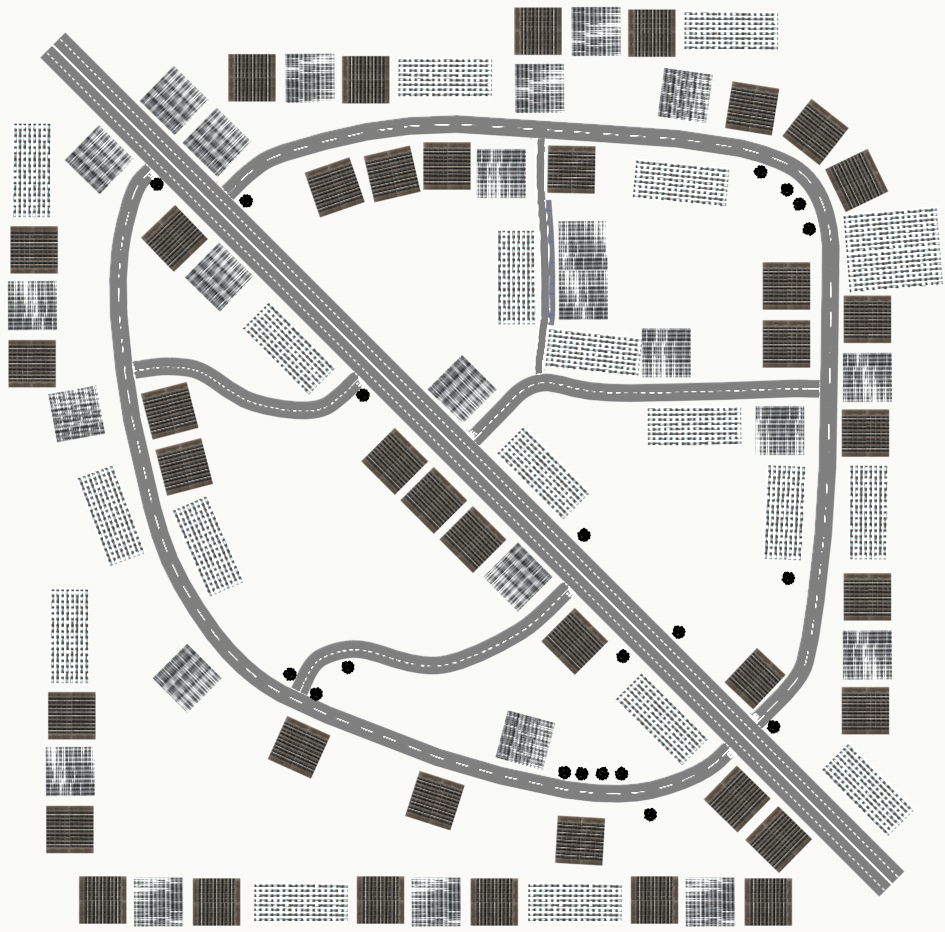
\includegraphics[scale=0.3]{src/CityWorld_map.png}
\caption{Karte der Stadtszene} % Titel der Grafik
\label{CityWorld_map} % Labelname
\end{figure}
Um die erstellte Stadtszene gut dokumentieren zu können, zeigt Abbildung \ref{CityWorld_map} eine Übersichtskarte. Die grosse vierspurige Strasse die sich von oben links nach unten rechts durch die gesamte Szene zieht ist eine rechteckige Ebene. Die ebene ist mit einer Textur versehen, die die vier Spuren mit einer Sicherheitelinie in der Mitte darstellt. Die Textur ist jedoch nicht so lange wie die gesammte Strasse. Sie hat nur die Länge von einmal einem Stück mit dem Strich der gestrichelten Sicherheitslinie, die die beiden Spuren die in die gleiche Richtung fahren trennt, und einmal ein Stück ohne dem Strich. Die Textur wird auf der Ebene immer wieder wiederhohlt. Auch bei allen anderen Strassen ist die Textur nur ein kurz und wird wiederholt. Ein Beispiel für eine solche Strassentextur ist in der Abbildung \ref{examples_street_textures} zu finden. \\
\begin{figure}[htbp]
\centering 
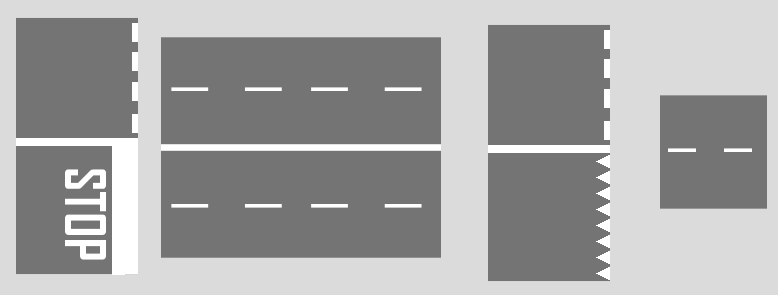
\includegraphics[scale=0.6]{src/examples_street_textures.png}
\caption{Beispiele von Strassentexturen} % Titel der Grafik
\label{examples_street_textures} % Labelname
\end{figure}
Die Strassen mit Kurven werden mit \glspl{spline} beschrieben. Eine Linie wird der \gls{spline} entlangeführt um die Breite einer Strasse zu erhalten. Die Textur der Strasse wird auf dieses, so zusammengefügte, Objekt gelegt. Der Abschluss solcher geschwungenen Strassen bilden wiederum rechteckige Ebenen. Diese erhalten die Textur einer Stoplinie mit Beschriftung auf der Strasse oder den vielen Dreieckigen Zeichen für kein Vortritt wie in Abbildung \ref{examples_street_textures} gezeigt. \\
Zusätzlich zu den Symbolen auf der Strasse, werden noch Verkehrsschilderobjekte in die Szene geladen. Die Abbildung \ref{screenshot_trafficsignal} zeigt ein Beipiel eines solchen Objektes. \\
\begin{figure}[htbp]
\centering 
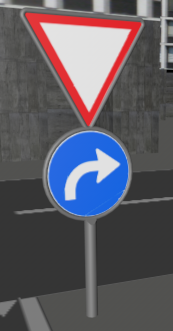
\includegraphics[scale=0.6]{src/screenshot_trafficsignal.png}
\caption{Beispiele eines Verkehrssignals} % Titel der Grafik
\label{screenshot_trafficsignal} % Labelname
\end{figure}

Die Häuser der Stadt sind einfache Blöcke die mit einer Textur von vielen Fenstern versehen werden. Insgesammt sind drei Gebäudetypen, wie in Abbildung \ref{screenshot_buildings} dargestellt,  vorhanden. Diese drei Typen werden einzeln dubliziert eventuell gedreht und in der Szene verteilt. Zusätzlich wird das ETH Zürich Gebäude in der Szene geladen. Dieses Gebäudemodel wurde aus dem Google 3D Warehouse heruntergeladen. Das Objekt wurde in google SketchUp bearbeitet und als eigenes Objekt abgespeichert. Die Bearbeitung heinhaltet vor allem die neuberechnung der Oberflächennormalen und das entfernen der Bodenplatte auf der die ETH Zürich gestanden hat. Die Texturen mussten manuell übernommen werden. Das ETH Objekt wird in die Szene geladen, skaliert und mit x- und y-Koordinaten plaziert. 
\begin{figure}[htbp]
\centering 
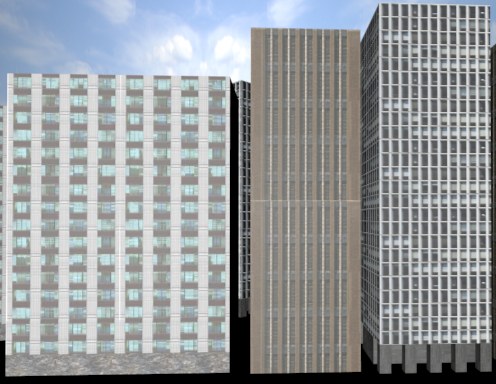
\includegraphics[scale=0.4]{src/screenshot_buildings.png}
\caption{Drei verschidene Gebäudetypen} % Titel der Grafik
\label{screenshot_buildings} % Labelname
\end{figure}
Um der Szene ein bisschen Farbe zu verleihen sind noch Bäume, wie in Abbildung \ref{screenshot_tree} in der Szene vorhanden. Ein Baum besteht aus einem Stamm mit einer Holztextur und einer Krone. Die Krone ist eine zufällig generierte Landschaft die zu einer Kugel geformt wird. Dadurch entstehen die verschiedenartigen Aus- und Einbuchtungen in der Baumkrone. Um die Illusion vollständig zu machen wird darauf eine Textur mit Blättern gelegt.\\

\begin{figure}[htbp]
\centering 
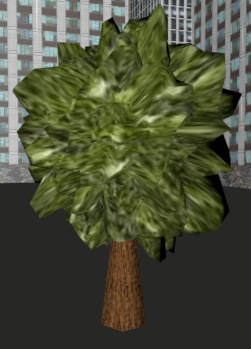
\includegraphics[scale=0.4]{src/screenshot_tree.png}
\caption{Baum} % Titel der Grafik
\label{screenshot_tree} % Labelname
\end{figure}

\subsubsection{Erstellung der Berglandschaft mit Tunnels}
Um die Berglandschaft zu generieren gibt es im Cinema4D ein eigens dafür vorgesehenes Objekt. Durch die Konfiguration des Landschaftsobjekt kann die Höhe und Anzahl der Erhöhungen und Vertiefungen festgelegt werden. Die Strasse in der Berglandschaft wird änlich gemacht wie in der Stadtszene. Zusätzlich wird aber der \gls{spline} ein halber Zilinder mitgegeben der ihr entlangfährt. Der halbe Zilinder wird mit einer Operation versehen damit er, an den Orten an denen die Strasse in der in der Landschaft befindet, diese ausschneidet und ein Tunnel generiert. Die Wand des Tunnels wird mit einer Betonplattenstruktur, wie sie in Abbildung \ref{texture_concretetiles} zeigt, versehen. Die Berglandschaft selbst wird mit einer \gls{seamless} Felsentexture versehen. 
\begin{figure}[htbp]
\centering 
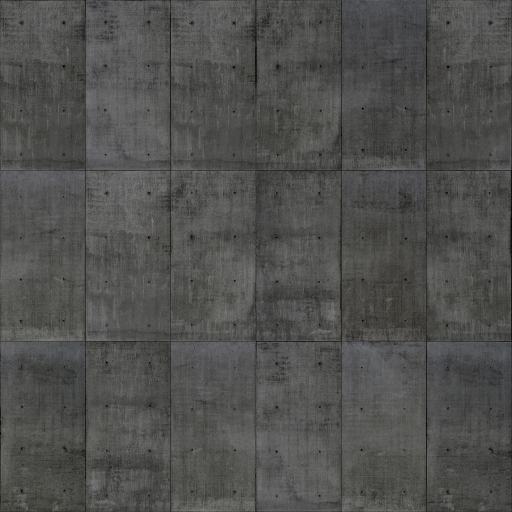
\includegraphics[scale=0.6]{src/texture_concretetiles.png}
\caption{Tunnelwandtextur} % Titel der Grafik
\label{texture_concretetiles} % Labelname
\end{figure}

\subsubsection{Eigenes Fahrerkabine und Geschwindigkeit}
Für die Darstellung eines Autos wurde aus dem Google 3D Warehouse ein Mini Cooper geladen. Wie in Abbildung \ref{screenshot_minicooper} zu sehen, wird dieser aus der Perspektive einer dritten Person betrachtet. Beim Rückwärtsfahren wird die Kamera um das Fahrzeug gedreht, so dass man nach hinten sehen kann. Mit der Taste V auf der Tastatur kann die Ansicht in das innere des Fahrzeugs gewechselt werden. Zu Beginn wirde die Kamera lediglich in das innere des Mini Coopers versetzt, dorthin wo der Kopf des Fahrers in etwa sein sollte. In einem zweiten Schritt wurde jedoch ein eigenes Fahrerkabine designed. Dies war vorallem deshalb notwendig, um eine Geschwindigkeitsanzeige implementieren zu können. Wie die Abbildung \ref{screenshot_cockpit} veranschaulicht, ist die Geschwindigkeitsanzeige die mittlere der drei Anzeigen. Sie besteht aus zwei Objekten. Eines der Objekte ist die gesamte Innenansicht selbst und das zweite Objekt ist der rote Zeiger der Geschwindigkeitsanzeige. Dieser wird an der richtigen Stelle Plaziert und wird je nach Geschwindigkeit gedreht. Somit sind zwei Ansichten möglich. Die Sicht des Fahrers mit der eigens dafür erstellten Fahrerkabine und die Aussenansicht in der der Mini Cooper angezeigt wird.\\
Um die Geschwindigkeit des Fahrzeuges herauszufinden, wurde im Cinema4D, in dem alle Szenen erstellt wurden, mit reellen Werten gearbeitet. So wurden Strassen wirklich sechs Meter breit modeliert. Somit konnte auch die Länge der Strasse festgelegt werden. Um die Geschwindigkeit zu ermitteln, wurde in Cinema4D eine Distanz abgemessen und diese mit verschiedenen Konstanten Geschwindigkeiten abgefahren und die Zeit gemessen. Die interne Geschwindigkeit im Programm wird mit einem Faktor in die tatsächliche Geschwindigkeit umgerechnet. Diese kann dann auf dem Tachometer angezeigt werden.\\

\subsection{Hautpprogramm}


%Sequenzdiagramm
%Blockdiagramm

